\documentclass{article}
\usepackage{graphicx}
\usepackage{amsmath}
\usepackage{geometry}
\usepackage{tikz}
\usepackage{hyperref}
\usetikzlibrary{shapes.geometric, arrows, positioning, fit, calc}
\geometry{a4paper, margin=1in}

\title{MCUMotionNet: A Lightweight, Two-Stage Architecture for Real-Time Object Tracking on Memory-Constrained Microcontrollers}
\author{Sébastien Campion}
\date{\today}

\begin{document}

\maketitle

\begin{abstract}
The proliferation of Tiny Machine Learning (TinyML) has pushed the boundaries of what is possible on low-power, resource-constrained microcontrollers (MCUs). However, complex tasks like real-time video analysis and object tracking remain a significant challenge due to strict memory and computational limits. This paper introduces MCUMotionNet, a novel two-stage deep learning architecture designed for real-time target tracking on MCUs with as little as 512KB of RAM. The architecture first employs a highly efficient object detector based on a truncated MobileNetV2 backbone and a Faster Objects, More Objects (FOMO) head to locate target centroids. Subsequently, a recurrent neural network (RNN) head processes temporal sequences of features to predict the necessary camera motion to keep a target in frame. We describe the model's application in tracking a handball player to automatically control a panoramic camera turret. We detail the experimental setup, including various configurations of the RNN head, which were trained on the Leonardo EuroHPC supercomputer to evaluate the trade-off between model complexity and tracking performance. The results demonstrate the viability of our approach for deploying sophisticated, real-time video-based tracking systems on edge devices.
\end{abstract}

\section{Introduction}
The Internet of Things (IoT) has led to an explosion of smart devices, creating a demand for processing data directly at the source, a paradigm known as edge computing. Tiny Machine Learning (TinyML) represents the cutting edge of this trend, focusing on the deployment of machine learning models on microcontrollers (MCUs) \cite{tinyml_survey_2}. These devices are characterized by their low cost, low power consumption, and minimal memory and processing resources, often having less than 1MB of RAM.

While TinyML has seen success in applications like keyword spotting and simple anomaly detection, tasks involving real-time video streams, such as object tracking, have remained largely out of reach. Traditional deep learning models for object detection and tracking are notoriously resource-intensive. This paper addresses the challenge of implementing a real-time, video-based tracking system on a severely constrained MCU, specifically targeting an ESP32-S3 with under 512KB of available RAM.

Our use case is the automated control of a camera turret designed to follow a player during a handball match. This requires not only detecting the player in each frame but also understanding their motion over time to predict the correct camera movement. To solve this, we propose MCUMotionNet, a specialized neural network architecture that combines efficient object detection with temporal sequence processing.\footnote{The source code for this project is available at: \url{https://github.com/scampion/MCUMotionNet}} The key contributions of this work are:
\begin{itemize}
    \item A novel two-stage architecture combining a MobileNetV2-FOMO detector with a lightweight RNN head for motion prediction.
    \item A demonstration of a complete system for real-time object tracking suitable for memory-constrained MCUs.
    \item An analysis of different model configurations to explore the performance-versus-complexity trade-off, with models trained on the Leonardo EuroHPC infrastructure.
\end{itemize}

\section{Related Work}
Our work builds upon several key advancements in efficient deep learning.

\textbf{MobileNetV2:} The MobileNet family of architectures is a cornerstone of efficient deep learning. MobileNetV2, in particular, introduced inverted residuals and linear bottlenecks, providing a powerful yet lightweight feature extractor for mobile and edge devices \cite{mobilenetv2}. We use a truncated version of MobileNetV2 as the backbone of our object detector.

\textbf{FOMO (Faster Objects, More Objects):} For object detection on the edge, traditional models that rely on bounding box prediction are often too slow. The FOMO paradigm, introduced by Edge Impulse, reframes object detection as a classification problem on a grid of the image \cite{fomo_edgeimpulse}. Instead of predicting bounding boxes, it identifies the centroids of objects. This simplification dramatically reduces computational load and model size, making it ideal for MCU-based applications.

\textbf{TinyML:} The field of TinyML is dedicated to optimizing machine learning models and systems for deployment on microcontrollers. This involves techniques like quantization, pruning, and the design of novel, hardware-aware neural network architectures. Several surveys document the rapid progress and challenges in this domain \cite{tinyml_survey_1, tinyml_survey_2}. MCUMotionNet is a practical application of TinyML principles to the complex problem of video analysis.

\section{MCUMotionNet Architecture}
MCUMotionNet is a two-stage, multi-head model designed to process a sequence of images and produce two distinct outputs: an object detection heatmap for the current frame and a motion prediction value based on the sequence. The architecture is detailed in the `create_fomo_td_with_rnn_combined_model` function in our codebase and visualized in Figure \ref{fig:architecture}.

\begin{figure}[h!]
\centering
\resizebox{\textwidth}{!}{%
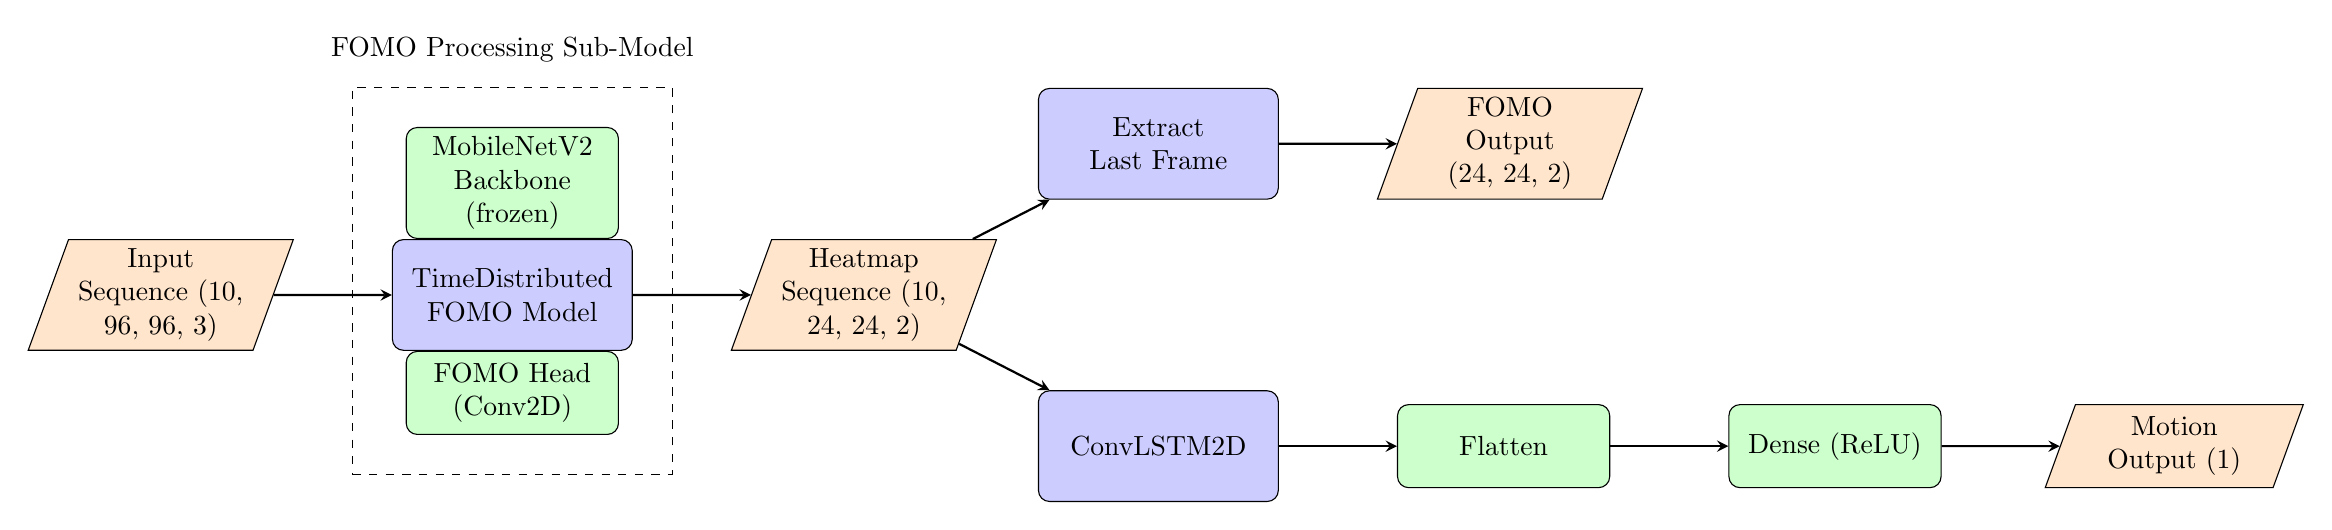
\begin{tikzpicture}[
    node distance=0.5cm and 1.5cm,
    block/.style={rectangle, draw, fill=blue!20, text width=8em, text centered, rounded corners, minimum height=4em},
    smallblock/.style={rectangle, draw, fill=green!20, text width=7em, text centered, rounded corners, minimum height=3em},
    arrow/.style={thick,->,>=stealth},
    line/.style={thick,-},
    io/.style={trapezium, trapezium left angle=70, trapezium right angle=110, draw, fill=orange!20, text width=6em, text centered, minimum height=3em},
    container/.style={rectangle, draw, dashed, inner sep=0.5cm}
]

% Nodes

\node[io] (input) {Input Sequence (10, 96, 96, 3)};

% TimeDistributed FOMO Model

\node[block, right=of input] (td_fomo) {TimeDistributed FOMO Model};

\node[smallblock, above=of td_fomo, yshift=-0.5cm] (fomo_backbone) {MobileNetV2 Backbone (frozen)};

\node[smallblock, below=of td_fomo, yshift=0.5cm] (fomo_head) {FOMO Head (Conv2D)};

% Dashed box for the sub-model

\node[container, fit=(fomo_backbone) (td_fomo) (fomo_head), label={[yshift=0.2cm]above:FOMO Processing Sub-Model}] (fomo_container) {};

\draw[arrow] (input) -- (td_fomo);

% Sequence Output

\node[io, right=of td_fomo] (seq_output) {Heatmap Sequence (10, 24, 24, 2)};
\draw[arrow] (td_fomo) -- (seq_output);

% Branch 1: FOMO Output

\node[block, above right=of seq_output] (lambda) {Extract Last Frame};

\node[io, right=of lambda] (fomo_output) {FOMO Output (24, 24, 2)};
\draw[arrow] (seq_output) -- (lambda);
\draw[arrow] (lambda) -- (fomo_output);

% Branch 2: Motion Prediction

\node[block, below right=of seq_output] (convlstm) {ConvLSTM2D};

\node[smallblock, right=of convlstm] (flatten) {Flatten};

\node[smallblock, right=of flatten] (dense) {Dense (ReLU)};

\node[io, right=of dense] (motion_output) {Motion Output (1)};

\draw[arrow] (seq_output) -- (convlstm);
\draw[arrow] (convlstm) -- (flatten);
\draw[arrow] (flatten) -- (dense);
\draw[arrow] (dense) -- (motion_output);

\end{tikzpicture}
}
\caption{The MCUMotionNet architecture. A TimeDistributed FOMO model processes an input sequence of 10 frames. The output splits into two heads: one extracts the final FOMO heatmap for object detection, and the other uses a ConvLSTM2D layer to process the full sequence for motion prediction.}
\label{fig:architecture}
\end{figure}

\subsection{Stage 1: FOMO-based Person Detector}
The first stage is a person detector based on the FOMO architecture. It is designed to be applied to each frame of an input video sequence.
\begin{itemize}
    \item \textbf{Backbone:} We use a MobileNetV2 model with a width multiplier (`alpha`) of 0.35 as the feature extractor. To keep the model small and increase the output resolution of the feature map, we truncate the backbone at the `block_3_expand_relu` layer. This results in a feature map with a spatial reduction factor of 4 (e.g., a 96x96 image produces a 24x24 feature map).
    \item \textbf{Head:} A simple convolutional head is attached to the backbone output. It consists of a 1x1 convolution to process the features, followed by another 1x1 convolution that produces a final heatmap. This heatmap has dimensions corresponding to the feature map grid (e.g., 24x24), with a channel depth equal to the number of classes plus one for the background. Each cell in the grid represents a classification of whether an object's centroid is present at that location.
\end{itemize}
This entire FOMO model is encapsulated in a `TimeDistributed` layer, allowing it to be applied independently to each of the 10 frames in the input sequence.

\subsection{Stage 2: RNN Motion Prediction Head}
The second stage is an RNN that analyzes the temporal information contained within the sequence of feature maps generated by the FOMO stage.
\begin{itemize}
    \item \textbf{Input:} The RNN head takes the output of the `TimeDistributed` FOMO model as its input. This is a sequence of heatmaps of shape (10, 24, 24, 2), where 10 is the sequence length, (24, 24) is the grid size, and 2 is for the 'person' and 'background' classes.
    \item \textbf{Recurrent Layer:} A `ConvLSTM2D` layer processes this sequence. `ConvLSTM2D` is well-suited for spatiotemporal data as it maintains the spatial structure (2D grid) of the input while processing it sequentially. It processes the entire sequence and returns a single output feature map.
    \item \textbf{Output Layers:} The feature map from the `ConvLSTM2D` layer is flattened and passed through a `Dense` layer with a ReLU activation, followed by a final `Dense` output layer with a `tanh` activation. This final layer outputs a single continuous value between -1 and 1, representing the predicted camera motion (pan left/right).
\end{itemize}

\subsection{Combined Model and Training Strategy}
The final model has a single input for an image sequence and two outputs:
\begin{enumerate}
    \item \textbf{FOMO Output:} The object detection heatmap from the very last frame in the sequence.
    \item \textbf{Motion Output:} The motion prediction value from the RNN head.
\end{enumerate}
The training is performed in two stages. First, the FOMO person detector is trained separately on a dataset of annotated single images. Then, in the second stage, its weights are loaded into the combined model and frozen. Only the RNN head (ConvLSTM and Dense layers) is trained on sequences of video frames with corresponding motion labels. This strategy allows the model to first learn a robust visual representation and then learn the temporal dynamics for motion prediction.

\section{Experimental Setup}
All Stage 2 training experiments were conducted on the Leonardo EuroHPC supercomputer.

\subsection{Dataset and Preprocessing}
The training data consists of `.mp4` video files from handball matches. For each video, a corresponding `.csv` file provides frame-by-frame annotations for the required camera motion. The `Move_X` column from the CSV is used as the ground truth label for our motion prediction task. This value is clipped and normalized to the range [-1, 1].

Input frames are resized to 96x96 pixels and normalized. The model takes sequences of 10 consecutive frames as input.

\subsection{Training Process}
The RNN head of the combined model is trained using the Adam optimizer with an initial learning rate of 0.0005. The loss function for the motion prediction output is Mean Squared Error (MSE), as it is a regression task. We monitor the validation loss and use callbacks for early stopping, learning rate reduction on plateau, and model checkpointing.

\subsection{Model Variations}
To find the best balance between performance and model size, we defined a series of experiments, each with a different configuration for the RNN head. The complexity of the `ConvLSTM2D` layer (number of filters) and the subsequent `Dense` layer (number of units) were varied. The configurations are listed in Table \ref{tab:experiments}.

\begin{table}[h!]
\centering
\caption{Experimental Configurations for the MCUMotionNet RNN Head.}
\label{tab:experiments}
\begin{tabular}{|l|c|c|c|c|}
\hline
\textbf{Experiment Name} & \textbf{ConvLSTM Filters} & \textbf{Dense Units} & \textbf{Val MAE} & \textbf{Model Size (KB)} \\ \hline
extra\_small\_rnn & 2 & 4 & TBD & TBD \\
small\_rnn & 4 & 8 & TBD & TBD \\
medium\_rnn & 8 & 16 & TBD & TBD \\
large\_rnn & 16 & 16 & TBD & TBD \\
extra\_large\_rnn & 32 & 32 & TBD & TBD \\ \hline
\end{tabular}
\end{table}

\section{Results and Discussion}
The training logs for the experiments listed in Table \ref{tab:experiments} were generated on the Leonardo supercomputer and are stored in the `logs_leo/` directory. A full quantitative analysis requires parsing these TensorBoard event files to extract the final validation metrics (e.g., Mean Absolute Error) and calculating the precise final model size for each configuration after quantization.

However, the experimental design allows us to discuss the expected trade-offs. The "extra\_small\_rnn" configuration is expected to produce the smallest and fastest model, making it the most likely candidate to fit within the strict 512KB RAM limit of the target MCU. As we move towards the "extra\_large\_rnn" configuration, the model's capacity to learn complex temporal patterns increases, which should lead to lower validation error and more accurate tracking. This increased complexity, however, comes at the cost of a larger model size and higher computational requirements.

The goal of this experimental sweep is to identify the "sweet spot": the simplest model configuration that provides "good enough" tracking performance for the handball use case while comfortably meeting the hardware constraints.

\section{Conclusion}
This paper presented MCUMotionNet, a lightweight, two-stage neural network architecture for real-time object tracking on resource-constrained microcontrollers. By combining a highly efficient FOMO-based object detector with a temporal RNN, our model can perform both object localization and motion prediction, making it suitable for controlling an automated camera turret. We have detailed the architecture, the two-stage training methodology, and the experimental framework used to evaluate different model complexities.

The work demonstrates a clear path toward enabling sophisticated, real-time video analysis on the smallest of edge devices. Future work will involve completing the quantitative analysis of the experimental results, quantizing the best-performing model, and deploying it on the target ESP32-S3 hardware to measure real-world performance and power consumption.

\begin{thebibliography}{9}

\bibitem{mobilenetv2}
Sandler, M., Howard, A., Zhu, M., Zhmoginov, A., & Chen, L. C. (2018).
\textit{MobileNetV2: Inverted Residuals and Linear Bottlenecks}.
arXiv preprint arXiv:1801.04381.

\bibitem{fomo_edgeimpulse}
Edge Impulse. (2022).
\textit{Introducing FOMO: Faster Objects, More Objects}.
Retrieved from Edge Impulse official documentation and blog.

\bibitem{tinyml_survey_1}
Cai, H., Gan, C., & Han, S. (2024).
\textit{From Tiny Machine Learning to Tiny Deep Learning: A Survey}.
arXiv preprint arXiv:2405.07722.

\bibitem{tinyml_survey_2}
Di Mauro, D., et al. (2024).
\textit{A Machine Learning-oriented Survey on Tiny Machine Learning}.
arXiv preprint arXiv:2402.17796.

\end{thebibliography}

\end{document}


